\documentclass[intro-breve-latex.tex]{subfiles}
\begin{document}

\chapter{Haciendo un documento básico desde cero}
En primera vamos a ver la estructura y características generales de \LaTeX{}.
A diferencia de MS Word, \LaTeX{} no es un generador WYSIWYG,%
\footnote{en. \textit{what you see is what you get}; lo que ves es lo que obtienes.}
sino que se escribe mediante texto en un archivo de texto y un lenguaje de marcado.
No se confundan, \LaTeX{} \textbf{no} es un lenguaje de programación, y no se parece a uno, sino que es como escribir texto común con comandos entre medio.

\section{<<Hola mundo>>}
Los comandos suelen tener esta estructura \lstinline|\comando{¬opciones¬}| donde la información obligatoria para el
comando suele ir entre llaves \texttt{\{\}} a los que llamaremos \textit{campos obligatorios}, mientras que la
información opcional suele ir entre corchetes \texttt{[]}. Todo documento comienza así:
\begin{lstlisting}
\documentclass[¬opciones¬]{¬tipo de documento¬}
\end{lstlisting}
Por el momento en las opciones incluiremos el tamaño normal de letra que es 10, 11 o 12pt y el tipo de documento será
\texttt{article} o \texttt{book} según lo que se desee escribir.

Luego viene un comando de la forma:
\begin{lstlisting}
\begin{document}
Hola mundo.
\end{document}
\end{lstlisting}
Varios comandos tendran la misma estructura, a estos les llamaremos \textit{entornos} y a la parte de \texttt{document}
su <<tag>>.
El entorno \texttt{document} señala todo lo perteciente al contenido del archivo. Todo lo que esté fuera de este entorno
(en particular antes de él) le diremos la \textit{cabecera} del documento. Debería compilar este archivo básico para
corroborar que su instalación de \LaTeX{} ha sido exitosa. Varios programas (como \TeX{}Maker) tienen compiladores
incluidos, pero si se interesa en hacerlo por la terminal puede ver el apéndice.

\textbf{Paquetes.}
Igual que los lenguajes de programación permiten añadir módulos para añadir funciones (como \texttt{<stdio.h>} en
\texttt{C}, o \texttt{numpy} en \texttt{Python}), \LaTeX{} ocupa paquetes que se incluyen en la cabecera, de momento
añadiremos dos:
\begin{lstlisting}
\usepackage[spanish]{babel}
\usepackage[utf8]{inputenc}
\end{lstlisting}
El primero le indica a \LaTeX{} que estamos escribiendo en español, para traducir texto del documento como escribir
<<Capítulo>> en lugar de <<Chapter>>. El segundo le dice a \LaTeX{} que lea las tildes y otros caracteres especiales
(e.g. á, ñ, ç, etc.) sin problema.

\textbf{Título.}
(Casi) todo documento tiene cosas como título, autor y fecha, para incluirlos en \LaTeX{} debe ocupar
correspondientemente los siguientes comandos en la cabecera:
\begin{lstlisting}
\title{Mí título interesante}
\author{Yo}
\date{\today}
\end{lstlisting}
Nótese que en la fecha utilice el comando \lstinline|\today|, este lee la fecha del día en el computador y el paquete de
\texttt{babel} lo traduce al español, pero puede ocupar cualquier otra que se le antoje. Dentro del documento y antes
del resto del texto escriba este comando para generar el título estándar de \LaTeX{}:
\begin{lstlisting}
\maketitle
\end{lstlisting}

\textbf{Secciones.}
Todo texto suele dividirse en secciones. \LaTeX{} también, y además las enumera automáticamente. En un artículo la mayor
división es una sección, luego una subsección y luego una sub-subsección:
\begin{lstlisting}
\section{Esta es mi sección}
\subsection{Esta mi subsección}
\subsubsection{Esta mi sub-subsección}
\end{lstlisting}
Un libro también admite todos los comandos anteriores, pero la mayor distinción es un capítulo \lstinline|\chapter{...}|
y se pueden agrupar los capítulos en partes \lstinline|\part{...}|,
donde las últimas se enumeran con números romanos, pero a diferencia de los capítulos no son obligatorios.

\textbf{Cortes de línea.}
Cuando hay un salto entre punto aparte y el otro párrafo eso se dice un \textit{corte de línea}, lo que uno está
acostumbrado a hacer con la tecla \texttt{Enter} de vuestros teclados.
No obstante, en el código de \LaTeX{} puede notar que no genera efecto alguno, esto se debe a que en los lenguajes de
marcado se da esta precaución para evitar líneas excesivamente largas en el código.  Para hacer este corte hay varias
formas:
\lstinline|\\| suele ser el más común, y no genera sangría en la línea contigua; para hacer un corte con sangría puede
usar dos veces \texttt{Enter} en el código o usar el comando \lstinline|\par|.  La sangría se puede añadir con
\lstinline|\indent| y quitar con \lstinline|\noindent| de ser necesario.
Por último, si necesita forzar un corte de línea, para evitar la sobrecarga de caractéres por ejemplo, puede usar
\lstinline|\break|.
\begin{multicols}{2}
\begin{lstlisting}
Texto de ejemplo.\break
Texto de ejemplo.\\
Texto de ejemplo.\par
Texto de ejemplo.
\end{lstlisting}
Texto de ejemplo.\break
Texto de ejemplo.\\
Texto de ejemplo.\par
Texto de ejemplo.
\end{multicols}

\textbf{Comentarios.}
Los comentarios son partes del código que no se deben interpretar como tal, pero pueden ser útiles para el
lector/escritor del código.
Éstos comenzan con el carácter \% en cualquier parte:
% \begin{multicols}{2}
\begin{lstlisting}
{\scshape Texto de ejemplo.} % Ésto estará en "mayúsculas pequeñas"
\end{lstlisting}
{\scshape Texto de ejemplo.} % Ésto estará en "mayúsculas pequeñas"
% \end{multicols}

\textbf{Caracteres especiales.}
Sabemos que los comandos se inician con \lstinline|\|, por ende, ¿cómo se escribe dicho caracter de ser necesario en
\LaTeX{}?  Esta clase de caracteres se dicen \textit{especiales} pues cumplen una función por si solos y se pueden
escribir así:
\begin{figure}[!h]
	\centering
	\begin{tabular}{ll|ll}
		\hline \hline
		\lstinline|$\backslash$| & $\backslash$ & \lstinline|\_|           & \_ \\
		\lstinline|\%|           & \%           & \lstinline|\#|           & \# \\
		\lstinline|\$|           & \$           & \lstinline|\&|           & \& \\
		\lstinline|\{\}|         & \{\} \\
		\hline \hline
	\end{tabular}
\end{figure}

Además debe tener en consideración que las comillas en \LaTeX{} son también distintas para escribir algo ``así'' se
requiere \lstinline|``así''|.
Donde las dos primeras son tildes graves y las últimas son apostrofes.
O también para algo <<así>> se requiere \lstinline|<<así>>|.

\section{Formato de texto}
\textbf{Estilos.}
Uno suele cambiar el formato, e.g. a \textbf{negritas}, o \textit{cursivas}, para ello \LaTeX{} ocupa:
\begin{ltabular}{lll}
	\lstinline|\textup{Derecho}|    & \lstinline|\upshape|  & \textup{Derecho}\\
	\lstinline|\textit{Cursivas}|   & \lstinline|\itshape|  & \textit{Cursivas}\\
	\lstinline|\textsl{Inclinado}|  & \lstinline|\slshape|  & \textsl{Inclinado}\\
	\lstinline|\textsc{Versalitas}| & \lstinline|\scshape|  & \textsc{Versalitas}\\
	\hline
	\lstinline|\textmd{Mediano}|    & \lstinline|\mdseries| & \textmd{Mediano}\\
	\lstinline|\textbf{Negritas}|   & \lstinline|\bfseries| & \textbf{Negritas}\\
	\hline
	\lstinline|\textrm{Romano}|     & \lstinline|\rmfamily| & \textrm{Romano}\\
	\lstinline|\textsf{Sans-serif}| & \lstinline|\sffamily| & \textsf{Sans-serif}\\
	\lstinline|\texttt{Máquina}|    & \lstinline|\ttfamily| & \texttt{Máquina}\\
\end{ltabular}

El segundo tipo de comando es lo que se dice un \textit{modificador}, al usarlo modifica todo el entorno,%
\footnote{En realidad modifica el entorno restante, ya que el contenido dentro del mismo entorno que viene ántes del modificador no se ve afectado.}
e.g., \lstinline|{\scshape Texto de Ejemplo}| {\scshape Texto de Ejemplo}.

\textbf{Tamaños.} Para los tamaños de letra puedes usar un modificador o un entorno, ambos ocupan el mismo tag:
\begin{center}
	{\tiny tiny}
	{\scriptsize scriptsize}
	{\footnotesize footnotesize}
	{\small small}
	{\normalsize normalsize}\\
	{\large large}
	{\Large Large}
	{\LARGE LARGE}
	{\huge huge}
	{\Huge Huge}
\end{center}
Cambiar el tamaño de letra por defecto (de 10 a 12pt por ejemplo) afecta también los otros tamaños de letra.

\textbf{Alineación.} \LaTeX{} permite de dos formas el cambio de alineación de texto:
\begin{figure}[!h]
	\centering
	\begin{tabular}{lll}
		\hline \hline
		Alineación & Entorno             & Modificador \\
		\hline
		Izquierda  & \texttt{flushleft}  & \lstinline|\raggedright| \\
		Derecha    & \texttt{flushright} & \lstinline|\raggedleft| \\
		Centro     & \texttt{center}     & \lstinline|\centering| \\
		\hline \hline
	\end{tabular}
\end{figure}

\textbf{Colores.} Para admitir colores extra se debe importar el siguiente paquete en la cabecera:
\begin{lstlisting}
\usepackage{xcolor}
\end{lstlisting}
Para usarlo puedes escribir: \lstinline|{\color{red} texto en rojo}| {\color{red} texto en rojo} o\break
\lstinline|\textcolor{blue}{texto en azúl}| \textcolor{blue}{texto en azúl}. Los nombres de colores por defecto son:
\begin{multicols}{5}
	\noindent\ttfamily
	\colorbox{black}{\color{white} black}\\
	\colorbox{blue}{\color{white} blue}\\
	\colorbox{brown}{brown}\\
	\colorbox{cyan}{cyan}\\
	\colorbox{darkgray}{\color{white} darkgray}\\
	\colorbox{gray}{gray}\\
	\colorbox{green}{green}\\
	\colorbox{lightgray}{lightgray}\\
	\colorbox{lime}{lime}\\
	\colorbox{magenta}{magenta}\\
	\colorbox{olive}{olive}\\
	\colorbox{orange}{orange}\\
	\colorbox{pink}{pink}\\
	\colorbox{purple}{\color{white} purple}\\
	\colorbox{red}{red}\\
	\colorbox{teal}{teal}\\
	\colorbox{violet}{\color{white} violet}\\
	\colorbox{white}{white}\\
	\colorbox{yellow}{yellow}
\end{multicols}
Para poner colores en el fondo se utiliza \lstinline|\colorbox{cyan}{Así}| \colorbox{cyan}{Así}.
Además puedes utilizar un porcentaje de un color, por ejemplo, si sólo queremos usar el 50\% de negro podemos escribir
\lstinline|\colorbox{black!50}{esto}| \colorbox{black!50}{esto}, y si queremos usar 50\% azúl y el resto rojo
\lstinline|\colorbox{blue!50!red}{haga esto}| \colorbox{blue!50!red}{haga esto}.

Por sobre eso, usted puede definir nuevos colores en la cabecera:
\begin{lstlisting}
\definecolor{ejemplo}{HTML}{00c89c}
\end{lstlisting}
Donde lo de \texttt{HTML} indica que la forma de definir colores es mediante el llamado código hexadecimal o
\texttt{hex} para acortar.
Este suele ser el método más común de definir colores, en línea lo reconocerá pues ocupan el prefijo `\texttt{\#}',
e.g., \texttt{\color{sample}\#00c89c}.

\textbf{Acentos y caracteres especiales.}
Como indicamos al principio, el paquete \texttt{inputenc} con opción \texttt{utf8} permite incluir caracteres especiales
de otros idiomas indoeuropeos; no obstante, puede seguir siendo útil saber cómo incluirlos de manera indirecta.
% acentos; no obstante, puede seguir siendo útil saber cómo incluir acentos y otros caracteres de manera indirecta.
He aquí una lista de comandos:
\begin{center}
	\begin{tabular}{|ll|ll|ll|ll|}
		\hline
		\lstinline|\AA| & \AA & \lstinline|\aa| & \aa &
		\lstinline|\AE| & \AE & \lstinline|\ae| & \ae \\
		\lstinline|\DH| & \DH & \lstinline|\dh| & \dh &
		\lstinline|\DJ| & \DJ & \lstinline|\dj| & \dj \\
		\lstinline|\L|  & \L  & \lstinline|\l|  & \l &
		\lstinline|\NG| & \NG & \lstinline|\ng| & \ng \\
		\lstinline|\O|  & \O  & \lstinline|\o|  & \o &
		\lstinline|\OE| & \OE & \lstinline|\oe| & \oe \\
		\lstinline|\TH| & \TH & \lstinline|\th| & \th &
		\lstinline|\ss| & \ss & {} & {} \\
		\hline
	\end{tabular}
\end{center}

Y para los acentos:
\begin{center}\begin{tabular}{*{4}{|ll}|}
	\hline
	\lstinline|\"{A}\"{a}| & \"{A}\"{a} &
	\lstinline|\'{A}\'{a}| & \'{A}\'{a} &
	\lstinline|\.{A}\.{a}| & \.{A}\.{a} &
	\lstinline|\={A}\={a}| & \={A}\={a} \\
	\lstinline|\^{A}\^{a}| & \^{A}\^{a} &
	\lstinline|\`{A}\`{a}| & \`{A}\`{a} &
	\lstinline|\~{A}\~{a}| & \~{A}\~{a} &
	\lstinline|\b{A}\b{a}| & \b{A}\b{a} \\
	\lstinline|\c{A}\c{a}| & \c{A}\c{a} &
	\lstinline|\d{A}\d{a}| & \d{A}\d{a} &
	% \lstinline|\G{A}\G{a}| & \G{A}\G{a}
	% \lstinline|\h{A}\h{a}| & \h{A}\h{a}
	\lstinline|\H{A}\H{a}| & \H{A}\H{a} &
	\lstinline|\k{A}\k{a}| & \k{A}\k{a} \\
	\lstinline|\r{A}\r{a}| & \r{A}\r{a} &
	\lstinline|\t{A}\t{a}| & \t{A}\t{a} &
	\lstinline|\u{A}\u{a}| & \u{A}\u{a} &
	\lstinline|\v{A}\v{a}| & \v{A}\v{a} \\
	\hline
\end{tabular}\end{center}
Para los marcados con violeta, se requiere el uso de una fuente distinta de la estándar.
El siguiente código sirve:
\begin{lstlisting}
\usepackage[T1]{fontenc}
\end{lstlisting}
También cabe destacar la existencia de los comandos \lstinline|\i| y \lstinline|\j| que producen <<\i>> y <<\j>> resp.,
lo que es útil para acentos como \lstinline|\u\i| (\u\i).

\textbf{Varias columnas.}
Si usted quisiera, de forma global, tener un documento escrito en dos columnas, sólo basta agregar la opción
\texttt{twocolumn} en \lstinline|\documentclass|. No obstante, si desea hacerlo localmente, esto es, en una sola parte
del documento, debe importar el paquete:
\begin{lstlisting}
\usepackage{multicol}
\end{lstlisting}
y luego usar el entorno \texttt{multicols} seguido del número de columnas:
\begin{lstlisting}
\begin{multicols}{2}
	Muchos años después, frente al pelotón de fusilamiento, el coronel Aureliano Buendía...
\end{multicols}
\end{lstlisting}
\begin{multicols}{2}
	Muchos años después, frente al pelotón de fusilamiento, el coronel Aureliano Buendía había de recordar aquella
	tarde remota en que su padre lo llevó a conocer el hielo. Macondo era entonces una aldea de veinte\break casas de barro y cañabrava construidas a la orilla de un río de aguas diáfanas que se precipitaban
	por un lecho de piedras pulidas, blancas y enormes como huevos prehistóricos.
\end{multicols}
% Dicho sea de paso, para forzar un rompimiento no de página sino ahora \emph{de columna} empleamos el comando
% \lstinline|\columnbreak|.

\section{Notas, listas, figuras y tablas}
\textbf{Notas.}
\LaTeX{} admite dos tipos comúnes de notas: al pie de la página y al margen de ella. La primera se especifica con el
comando \lstinline|\footnote{Esta es una nota al pie de página.}|\footnote{Esta es una nota al pie de página.} mientras
que las notas de margen se hacen con \lstinline|\marginpar{Y ésta, una nota al margen.}|\marginpar{Y ésta, una nota al
margen.}. Para revertir el lugar se puede usar \lstinline|\reversemarginpar{...}|.

Para más información y mejor manejo de las notas al margen se recomienda revisar el paquete \texttt{marginnote}.

\subsection{Listas}
Se dividen en tres: numeradas, no numeradas y descripciones (similar a un glosario o diccionario).
Todas se definen por un entorno y sus elementos se diferencian por el comando \lstinline|\item|.
Para una lista enumerada el entorno utiliza el tag \texttt{enumerate}, las no numeradas el tag \texttt{itemize} y las
descripciones \texttt{description}.
En las descripciones, la palabra (o frase) de título se denota en el campo opcional de \lstinline|\item[¬Aquí...¬]|.
Por ejemplo:
\begin{lstlisting}[basicstyle=\footnotesize\ttfamily]
\begin{enumerate}
	\item Naranjas.
	\item Manzanas:
		\begin{itemize}
			\item Rojas.
			\item Verdes.
			\item Amarillas.
		\end{itemize}
	\item Bananas.
\end{enumerate}
\begin{description}
	\item[Fruta] Fruto comestible de ciertas plantas cultivadas; e.g., la pera, la guinda, la fresa, etc.
	\item[Verdura] Hortaliza, especialmente la de hojas verdes.
\end{description}
\end{lstlisting}
\begin{enumerate}
	\item Naranjas.
	\item Manzanas:
		\begin{itemize}
			\item Rojas.
			\item Verdes.
			\item Amarillas.
		\end{itemize}
	\item Bananas.
\end{enumerate}
\begin{description}
	\item[Fruta] Fruto comestible de ciertas plantas cultivadas; e.g., la pera, la guinda, la fresa, etc.
	\item[Verdura] Hortaliza, especialmente la de hojas verdes.
\end{description}

Una recomendación personal es usar el siguiente paquete:%
\footnote{En la versión anterior (26-06-21) se recomendaba \texttt{enumerate}, sin embargo, el mismo autor del paquete
recomienda en cambio usar \texttt{enumitem}. Vea \url{https://tex.stackexchange.com/a/519982}.}
\begin{lstlisting}
\usepackage[shortlabels]{enumitem}
\end{lstlisting}
que permite modificar de manera más sencilla las listas:
\begin{multicols}{2}
	\begin{lstlisting}[basicstyle=\footnotesize\ttfamily]
\begin{enumerate}[i)]
	\item Frutas.
	\begin{enumerate}[1.]
		\item Rojas.
		\begin{enumerate}[(a)]
			\item Manzana.
			\item Frutilla.
			\item Frambuesa.
		\end{enumerate}
		\item Verdes.
		\begin{enumerate}[(a)]
			\item Manzana.
			\item Pera.
			\item Sandía.
		\end{enumerate}
	\end{enumerate}
	\item Verduras.
	\begin{enumerate}[(a)]
		\item Lechuga.
		\item Repollo.
		\item Apio.
	\end{enumerate}
\end{enumerate}
	\end{lstlisting}

	\vfill\null
	\columnbreak

	\begin{enumerate}[i)]
		\item Frutas.
			\begin{enumerate}[1.]
				\item Rojas.
					\begin{enumerate}[(a)]
						\item Manzana.
						\item Frutilla.
						\item Frambuesa.
					\end{enumerate}
				\item Verdes.
					\begin{enumerate}[(a)]
						\item Manzana.
						\item Pera.
						\item Sandía.
					\end{enumerate}
			\end{enumerate}
		\item Verduras.
			\begin{enumerate}[(a)]
				\item Lechuga.
				\item Repollo.
				\item Apio.
			\end{enumerate}
	\end{enumerate}
\end{multicols}

\textbf{Figuras y tablas.}
Por defecto, \LaTeX{} no permite importar imágenes al documento por lo que se requiere importar el paquete:
\begin{lstlisting}
\usepackage{graphicx}
\end{lstlisting}
Luego para importar la figura (asumiendo que la imágen está en la misma carpeta que el archivo) se utiliza el siguiente comando:
\begin{lstlisting}
\includegraphics[¬opciones¬]{imagen.jpg}
\end{lstlisting}
En las opciones usualmente van especificaciones sobre el tamaño, verá que sin ella la figura se importa al máximo tamaño
para el cual no pierde detalle, para importarlo digamos a la mitad de su tamaño real puede usar \texttt{scale=.5}, pero
usualmente es mejor especificar directamente ya sea el largo (\texttt{width}) o el alto (\texttt{height}) del archivo
que debe hacerse en \texttt{cm}, \texttt{mm} o \texttt{in} (pulgadas). También podemos decirle que sea tan larga como el
tamaño del texto usando \lstinline|width=\textwidth|.

Para que la imagen este apartada del texto se incluye todo dentro de un entorno \texttt{figure} cuyo único propósito es
ese de decirle a \LaTeX{} que trate la imagen individualmente.
Dentro de él se recomienda centrar el texto (o en este caso el contenido) y al final del entorno se recomienda añadir
alguna forma de corte de línea para mejorar el formato.

\textbf{Posicionamiento.}
Para saber donde ubicar la imagen, \LaTeX{} utiliza los siguientes símbolos para abreviar:
\begin{ltabular}{lp{8cm}}
	\texttt{h} & Aproximadamente en el lugar donde se ubica en el código. \\
	\texttt{t} & En el tope de la página siguiente. \\
	\texttt{b} & En el fondo de la página actual. \\
	\texttt{p} & En la siguiente página, destinada exclusivamente para figuras. \\
	\texttt{!} & Fuerza la posición indicada. \\
\end{ltabular}

\textbf{Descripciones.}
Además las imágenes poseen descripciones cortas, estas pueden agregarse en \LaTeX{} dentro de un entorno \texttt{figure}
con el comando \lstinline|\caption{Mi descripción.}|, veamos un ejemplo donde se utiliza todo lo anterior:
\begin{lstlisting}
\begin{figure}[!h]
	\centering
	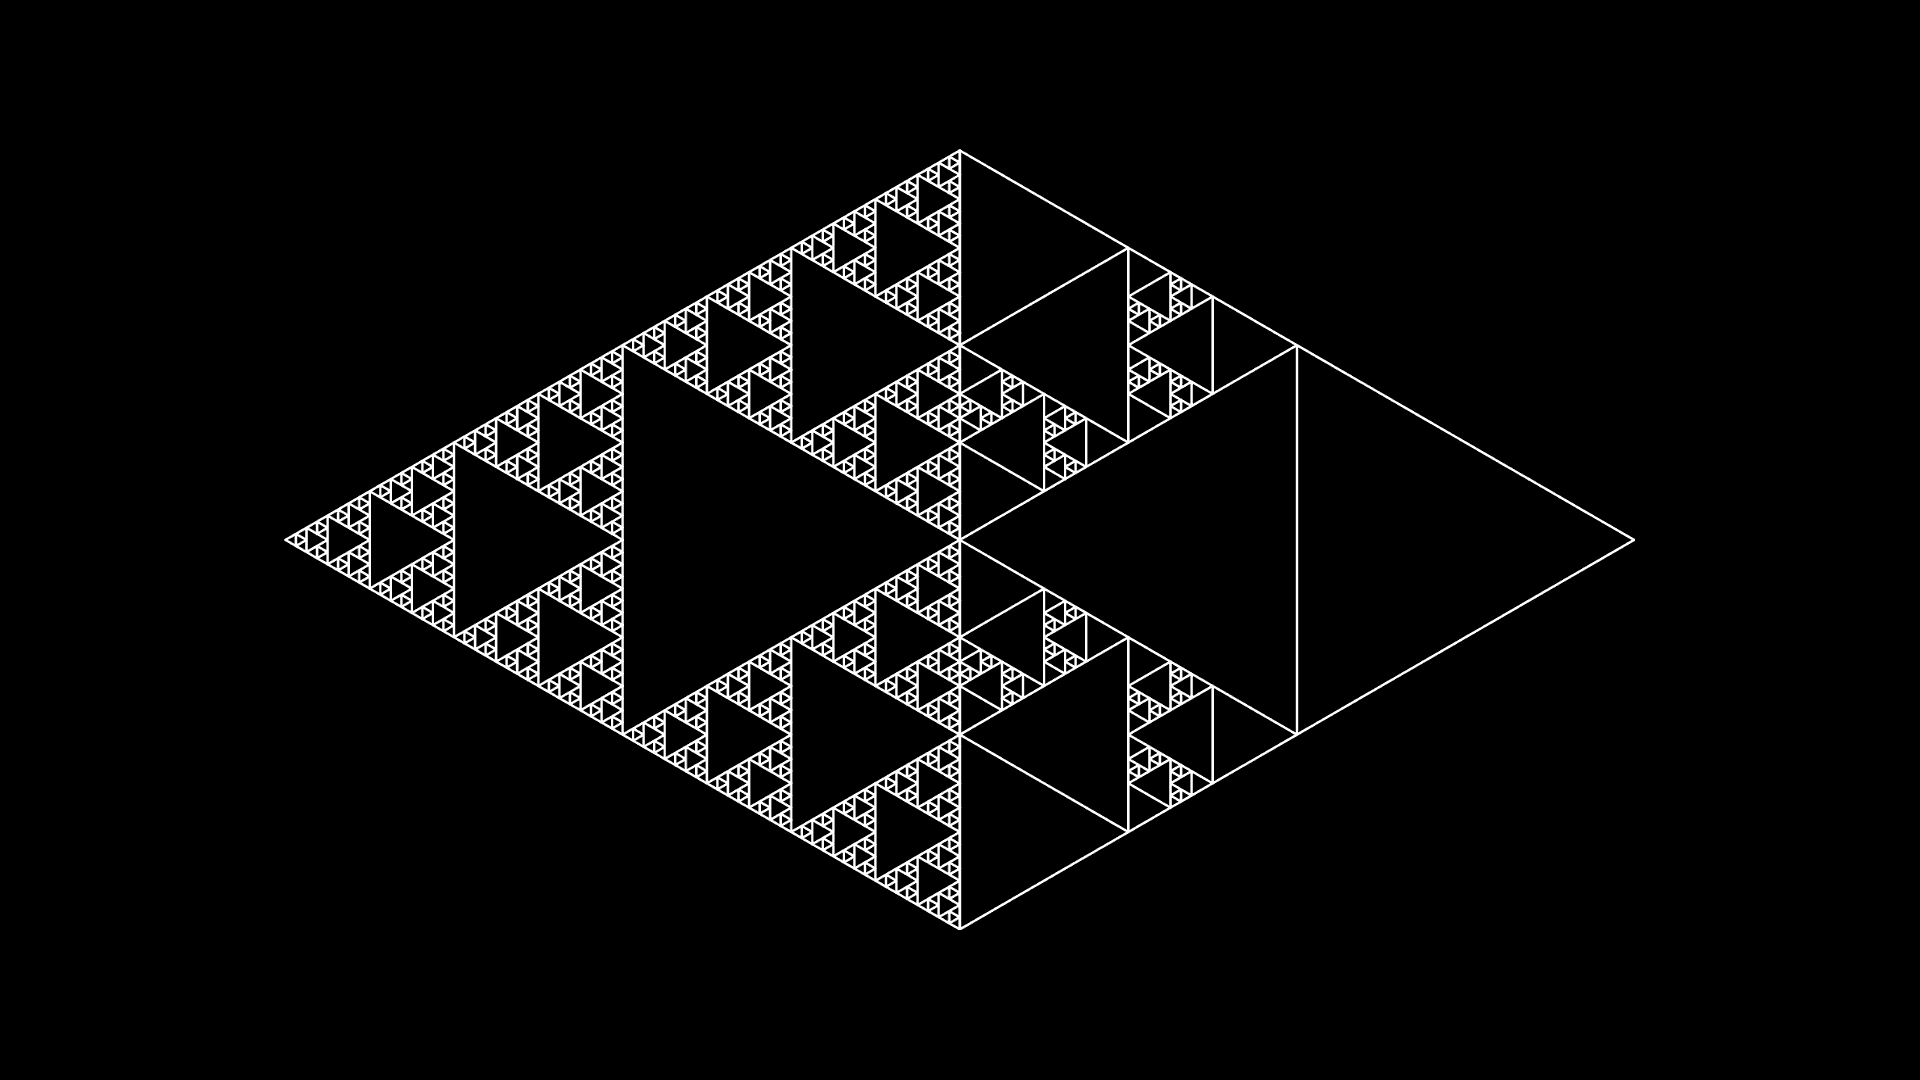
\includegraphics[width=6.5cm]{fractal.png}
	\caption{Un fractal}
\end{figure}
\end{lstlisting}
\begin{figure}[!h]
	\centering
	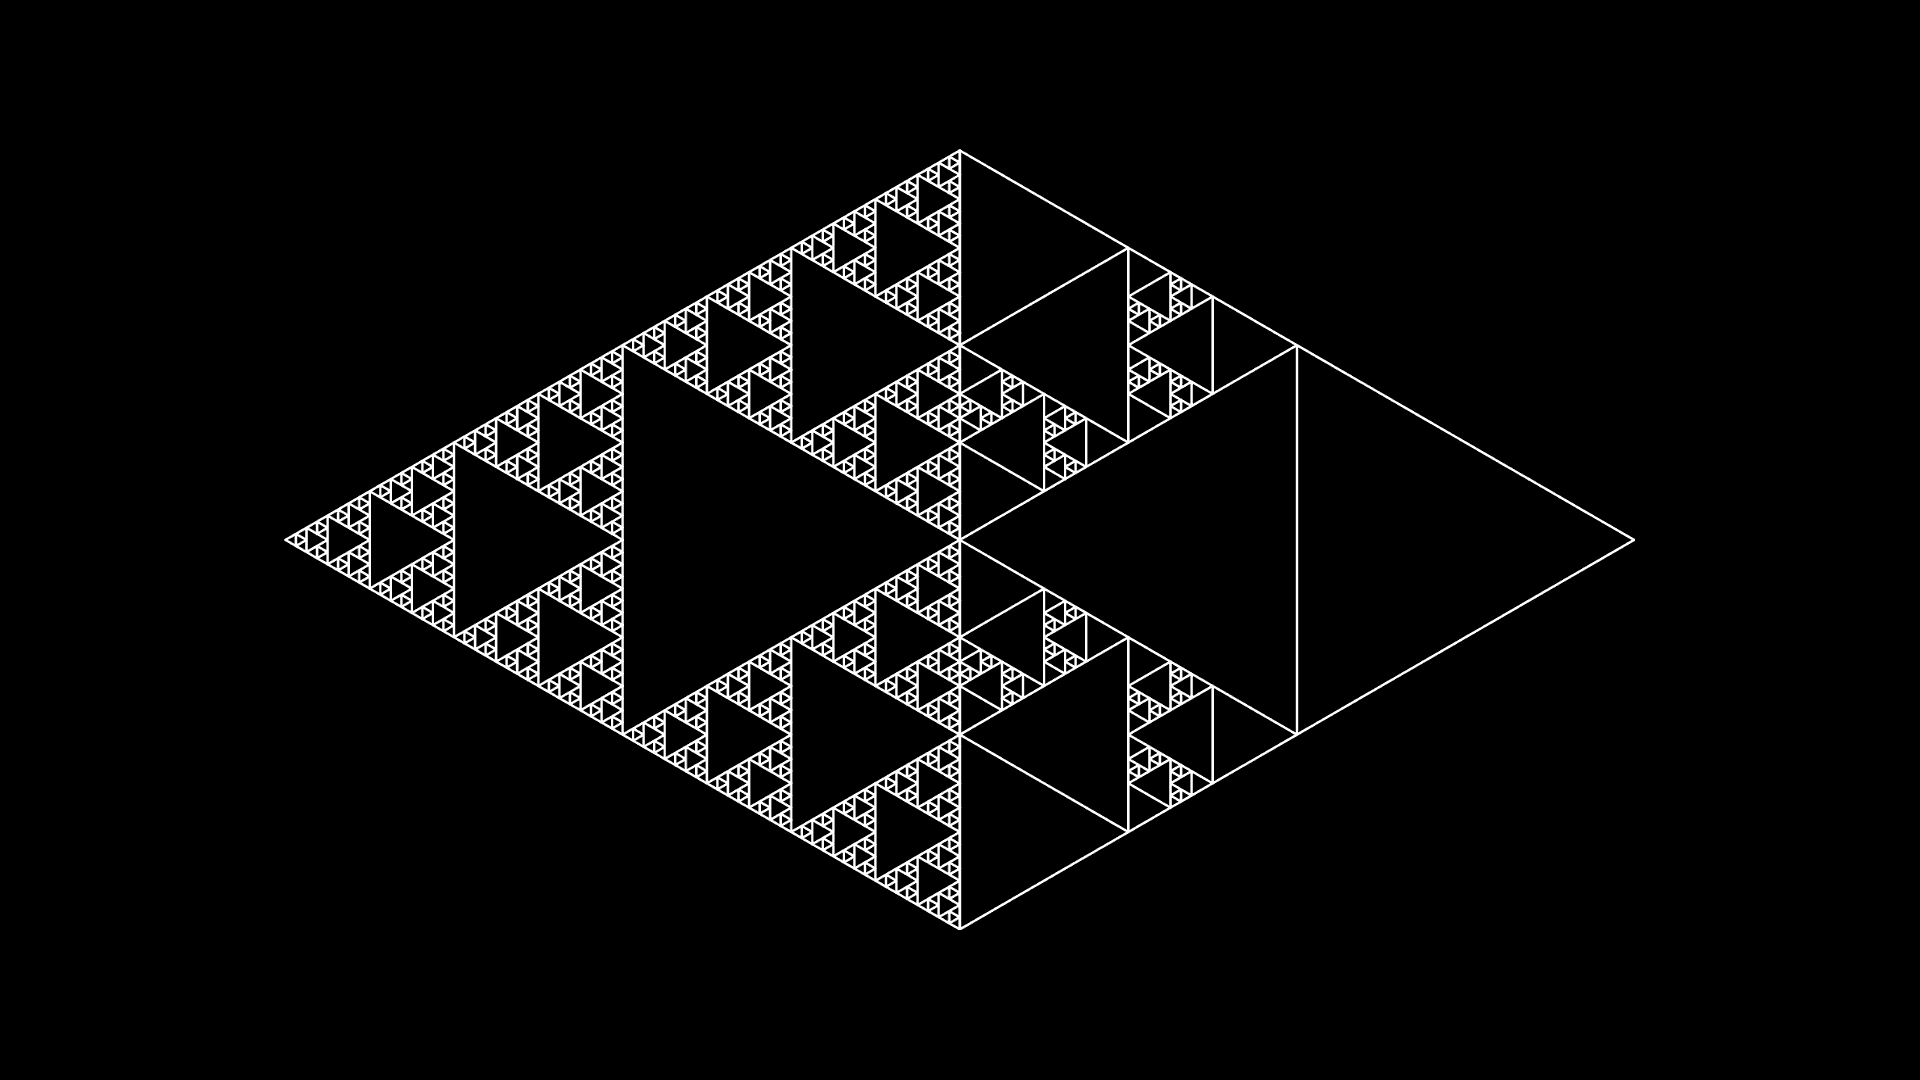
\includegraphics[width=6.5cm]{fractal.png}
	\caption{Un fractal}
\end{figure}

\textbf{Tablas.} Las tablas se definen así:
\begin{lstlisting}
\begin{tabular}{¬formato¬}
	...
\end{tabular}
\end{lstlisting}
Donde el \textit{formato} se define por lo siguiente:
\begin{ltabular}{lp{8cm}}
	\lstinline|l|	     & Celdas hacia la izquierda. \\
	\lstinline|c|	     & Celdas centradas. \\
	\lstinline|r|	     & Celdas hacia la derecha. \\
	\lstinline|p{¬longitud¬}| & Párrafo de cierta longitud. \\
	\lstinline|m{¬longitud¬}| & Como \texttt{p}, pero centrado verticalmente\textsuperscript{\dag}. \\
	\lstinline|b{¬longitud¬}| & Como \texttt{p}, pero verticalmente al fondo\textsuperscript{\dag}. \\
\end{ltabular}

Los marcados por \dag{} requieren del paquete \texttt{array}. Las celdas en una columna se separan por el símbolo \texttt{\&} y las columnas se separan por un corte de línea. Además \lstinline|\hline| genera una línea horizontal lo que puede ser útil. Tal como uno pone las figuras en un entorno \texttt{figure}, existe el entorno \texttt{table} para tablas que sirve para posicionar y añadir descripciones; funciona exactamente igual.
\begin{lstlisting}
\begin{table}[!h]
	\centering
	\begin{tabular}{|lcc|}
		\hline
		País & Contagios totales & Fallecidos totales \\
		\hline \hline
		Argentina & 201,919 & 3,667 \\
		Chile     & 361,493 & 9,707 \\
		Colombia  & 317,651 & 10,650 \\
		Peru      & 428,850 & 19,614 \\
		\hline
	\end{tabular}
	\caption{Estado Covid-19 (3 de agosto de 2020).}
\end{table}
\end{lstlisting}
\begin{table}[!h]
	\centering
	\begin{tabular}{|lcc|}
		\hline
		País & Contagios totales & Fallecidos totales \\
		\hline \hline
		Argentina & 201,919 & 3,667 \\
		Chile     & 361,493 & 9,707 \\
		Colombia  & 317,651 & 10,650 \\
		Peru      & 428,850 & 19,614 \\
		\hline
	\end{tabular}
	\caption{Estado Covid-19 (3 de agosto de 2020).}
\end{table}

Se puede agrupar un formato y repetir $n$ veces con la abreviación \lstinline|*{¬n¬}{¬formato¬}|. En el ejemplo anterior podríamos reemplazar la \lstinline|cc| por \lstinline|*{2}{c}|. Una celda puede usar el tamaño de varias dentro de la misma fila usando el comando \lstinline|\multicolumn{¬num¬}{¬form¬}{¬contenido¬}| donde \textit{num} es el número de columnas que abarca, y \textit{form} el formato de ella, e.g:
\begin{lstlisting}[basicstyle=\footnotesize\ttfamily]
\begin{table}[!h]
	\centering
	\begin{tabular}{|l|cc|}
		\hline
		País & Contagios totales & Nuevos contagios \\
		\hline \hline
		\multicolumn{3}{|c|}{\sffamily América} \\
		\hline
		EEUU        & 4,851,407 & +38,379 \\
		Brasil      & 2,736,298 & +2,621  \\
		\hline
		\multicolumn{3}{|c|}{\sffamily Europa} \\
		\hline
		Reino Unido & 305,623   & +928    \\
		Italia      & 248,229   & +159    \\
		\hline
	\end{tabular}
\end{table}
\end{lstlisting}
\begin{table}[!h]
	\centering
	\begin{tabular}{|l|cc|}
		\hline
		País & Contagios totales & Nuevos contagios \\
		\hline \hline
		\multicolumn{3}{|c|}{\sffamily América} \\
		\hline
		EEUU        & 4,851,407 & +38,379 \\
		Brasil      & 2,736,298 & +2,621  \\
		\hline
		\multicolumn{3}{|c|}{\sffamily Europa} \\
		\hline
		Reino Unido & 305,623   & +928    \\
		Italia      & 248,229   & +159    \\
		\hline
	\end{tabular}
\end{table}

Con el paquete \texttt{multirow} puedes combinar filas también mediante el comando \lstinline|\multirow{¬num¬}{¬longitud¬}{¬contenido¬}| (puedes usar \texttt{*} en el lugar de la longitud para ocupar todo lo disponible). Y puedes hacer líneas horizontales parciales desde el inicio de la $i$-ésima celda hasta el final de la $j$-ésima celda con \lstinline|\cline{¬i-j¬}|, e.g.:
\begin{lstlisting}[basicstyle=\footnotesize\ttfamily]
\begin{table}[!h]
	\centering
	\begin{tabular}{|l|lcc|}
		\cline{2-4}
		\multicolumn{1}{c|}{}    & País   & Contagios totales & Nuevos contagios \\
		\hline
		\multirow{2}{*}{América} & EEUU   & 4,851,407         & +38,379 \\
		\cline{2-4}
		{}                       & Brasil & 2,736,298         & +2,621  \\
		\hline
	\end{tabular}
\end{table}
\end{lstlisting}
\begin{table}[!h]
	\centering
	\begin{tabular}{|l|lcc|}
		\cline{2-4}
		\multicolumn{1}{c|}{}    & País   & Contagios totales & Nuevos contagios \\
		\hline
		\multirow{2}{*}{América} & EEUU   & 4,851,407         & +38,379 \\
		\cline{2-4}
		{}                       & Brasil & 2,736,298         & +2,621  \\
		\hline
	\end{tabular}
\end{table}
\textbf{Tablas entre páginas.} Por defecto \LaTeX{} no rompe una tabla entre páginas, sin importar cuan larga sea, para poder usar un \textit{tabla larga} se debe importar el paquete \texttt{longtable} que provee el entorno homónimo que funciona exactamente igual que \texttt{tabular}.

\section{Bibliografías, referencias cruzadas e índices}
\label{sec:crossref}
\LaTeX{} es bastante popular por su forma de tratar bibliografías, por lo cual vamos a enseñar como: En primer lugar, todas las referencias bibliográficas se guardan en otro archivo externo de extensión \texttt{.bib}. Para incluir una bibliografía debemos añadir el siguiente comando:
\begin{lstlisting}
\usepackage[backend=biber]{biblatex}
\addbibresource{¬mis-referencias¬.bib}
\end{lstlisting}
Y para compilarlo hay que compilar el documento una primera vez, luego compilar la bibliografía con \textit{biber} y luego una segunda vez. Esto se debe a que la primera vez le dice a \LaTeX{} que referencias crear, luego el compilador las crea con su respectivo formato y la última las incluye.

Las referencias se pueden buscar facilmente en páginas como \url{https://scholar.google.com/} y luego seleccionando obtener el formato en Bib\TeX{} o similar. En general toda referencia suele verse así:
\begin{lstlisting}
@book{gauss1966disquisitiones,
	title={Disquisitiones arithmeticae},
	author={Gauss, Carl Friedrich},
	volume={157},
	year={1966},
	publisher={Yale University Press}
}
\end{lstlisting}
Donde es bastante claro como funciona, la palabra \texttt{book} indica que la referencia es un libro, \texttt{gauss1966disquisitiones} es lo que le decimos una \textit{etiqueta}, i.e., una cadena de signos sin espacios que se utiliza para citar dentro del documento, luego el resto es claro. Lo único importante a saber es que en el campo del autor se recomienda anotar apellido, luego coma, luego nombre; y si hay más de uno separarlos por la palabra \texttt{and}, si hay muchos y se quiere utilizar algo para decir ``y otros'' (et al. en latín) se utiliza un \texttt{others} (Albert Einstein et al. sería \texttt{Einstein, Albert and others} para \LaTeX{}).

Usualmente se utiliza un solo archivo general para tener todas las referencias allí, luego, utilizando el ejemplo anterior, uno citaría un documento así:
\begin{lstlisting}
\cite{gauss1966disquisitiones}
\end{lstlisting}
Si se quiere que la cita este al pie de página uno ocupa \lstinline|\footcite{...}| y puedes citar varios documentos juntos separando las etiquetas por comas. Entre las referencias sólo aparecerán los trabajos citados. Para incluir un trabajo sin citarlo en la bibliografía debemos usar el comando \lstinline|\nocite{...}| donde las mismas reglas se aplican.
Si se quiere incluir a todas las referencias puedes escribir \lstinline|\nocite{*}|. 
Para imprimir las bibliografías se ocupa este comando:
\begin{lstlisting}
\printbibliography
\end{lstlisting}

\textbf{Sub-bibliografías y palabras clave.} No obstante, un problema que puede surgir al tratar bibliografías es que toman un capítulo (o sección si de un artículo se trata) entero cuando se imprimen, y un formato interesante es el de ciertos libros que usan bibliografía para cada capítulo, lo que por el momento parece una tarea imposible. Un problema similar es si queremos incluir muchos artículos a la vez, pero no todos y sólo queremos incluir los de un cierto tema. Para ambos la solución implica introducir el mismo concepto: palabras clave.

Dentro de la definición de libros en Bib\TeX{} se añade la categoría \texttt{keywords} (sí, plural) donde especifica las palabras clave separadas por comas. Tomemos el ejemplo del libro de Gauss y supongamos que le añadimos \lstinline|keywords={arithmetic}| donde tenemos varias referencias marcadas sobre el tema de \texttt{arithmetic} luego este comando:
\begin{lstlisting}
\printbibliography[keyword={arithmetic}]
\end{lstlisting}
Imprimirá sólo dichos artículos. Para el problema de las sub-bibliografías añada la opción de \texttt{subbibintoc}. Y para cambiarle el nombre puede usar la opción, \lstinline|heading={¬mi título¬}|.

\textbf{Referencias cruzadas.} Una de las ventajas de \LaTeX{} es que como genera automáticamente la numeración para las secciones, figuras y ecuaciones, se pueden referenciar de forma bastante sencilla, junto a uno de esos entornos se agrega el comando \lstinline|\label{¬etiqueta¬}| y luego se llama con \lstinline|\ref{¬etiqueta¬}| (puede requerir una compilación doble para funcionar adecuadamente), e.g:
\begin{lstlisting}[basicstyle=\footnotesize\ttfamily]
\section{Bibliografías, referencias cruzadas e índices}
\label{sec:crossref}
---------------------------------------------------
...similar a lo dicho en la sección \ref{sec:crossref}.
\end{lstlisting}
...similar a lo dicho en la sección \ref{sec:crossref}.

La parte de \texttt{sec:} es una costumbre decorativa, así como se suele usar \texttt{eq:} como prefijo para las ecuaciones, \texttt{fig:} para las figuras, etc. No es necesaria pero puede servir para ordenarse en el código fuente.

\textbf{Tablas de contenidos.} La tabla de contenidos no puede ser más fácil de implementar, sólo basta con el comando:
\begin{lstlisting}
\tableofcontents
\end{lstlisting}
Además se pueden usar \lstinline|\listoftables| y \lstinline|\listoffigures| para imprimir índices de las tablas y las figuras del documento (sólo ocupa las entradas  con descripciones, puedes hacer descripciones vacías para que esten numeradas).

\textbf{Hipervínculos.} Si ha descargado este documento notará que puede \textit{hacer click} en la referencia cruzada anterior que lo lleva a la página de inicio de la sección, lo mismo ocurre con todas las entradas de la tabla de contenidos y con los enlaces web, para ello es tan sencillo como agregar el siguiente paquete:
\begin{lstlisting}
\usepackage{hyperref}
\end{lstlisting}
Para añadir las entradas de las secciones al índice del pdf, agrega las opciones \texttt{bookmarks=true} y \texttt{bookmarksnumbered=true}. Aquí puedes añadir urls con el comando \lstinline|\url{¬url¬}| y \lstinline|\href{¬url¬}{¬texto¬}|; y referencias cruzadas extra con \lstinline|\hyperref{¬etiqueta¬}{¬texto¬}|.

\section{Configurar mi documento}
\label{sec:setup}
Esta sección es opcional, pero se recomienda bastante para mejorar su experiencia y efeciencia con \LaTeX{}:

\textbf{(Re) definir comandos.} Además de los comandos actuales, se pueden definir nuevos con \lstinline|\newcommand|, este va seguido del nombre del comando y luego del uso, e.g:
\begin{lstlisting}
\newcommand{\licencia}{Éste documento está bajo la licencia xyz (2020).}
---------------------------------------------------
\licencia
\end{lstlisting}
\begingroup
\newcommand{\licencia}{Éste documento está bajo la licencia xyz (2020).}
\licencia
\endgroup

Si quiere añadirle opciones al comando entonces debe poner un campo opcional con el número de opciones y luego referirse a ellas dentro de la definición como \lstinline|#1|, \lstinline|#2| y así:
\begin{lstlisting}
\newcommand{\licencia}[2]{Éste documento está bajo la licencia #2 (#1).}
---------------------------------------------------
\licencia{2019}{uvw}
\end{lstlisting}
\begingroup
\newcommand{\licencia}[2]{Éste documento está bajo la licencia #2 (#1).}
\licencia{2019}{uvw}
\endgroup

Además también puedes pasar argumentos opcionales, que toman el lugar del primer argumento si están dados y cuyo valor por defecto queda definido en el segundo campo opcional:
\begin{lstlisting}
\newcommand{\licencia}[2][2020]{Éste documento está bajo la licencia #2 (#1).}
---------------------------------------------------
\licencia{abc}\\
\licencia[1995]{def}
\end{lstlisting}
\begingroup
\newcommand{\licencia}[2][2020]{Éste documento está bajo la licencia #2 (#1).}
\licencia{abc}\\
\licencia[1995]{def}
\endgroup

Si un comando ya existe, \LaTeX{} tirará un error al tratar de sobreescribirlo, para poder hacerlo debes usar \lstinline|\renewcommand|, que funciona exactamente igual. Éste último también tira error si se trata de redefinir un comando que no ha sido definido antes.

\textbf{Definir entornos.}
Para definir entornos, se ocupan \lstinline|\newenvironment| y \lstinline|\renewenvironment| que funcionan exactamente
igual, sólo que en lugar de poner un comando pones el tag del entorno y al final se ocupan dos campos obligatorios que
determinan el código a ejecutar ántes y después del contenido del entorno. Pero todo uso de argumentos extra van en la
primera parte y no pueden ir al final, e.g:
\begin{lstlisting}
\newenvironment{demo}[1][$\bullet$]{#1 {\scshape Demostración:} }{\par\noindent}
---------------------------------------------------
\begin{demo}
	Esto se deduce de que el triángulo sea isóceles.
\end{demo}
\begin{demo}[(?)]
	Esto es obvio.
\end{demo}
\end{lstlisting}
\begin{demo}
	Esto se deduce de que el triángulo sea isóceles.
\end{demo}
\begin{demo}[(?)]
	Esto es obvio.
\end{demo}
\textbf{Plantillas.} Si usted ha seguido el texto hasta ahora, probando de todo lo que se menciona, es probable que la cabecera de su documento tenga hartas líneas y genere un poco de confusión, sin contar con el hecho de que si piensa hacer otro documento tendrá que copiar y pegar todo eso. Para esto existen las llamadas \textit{plantillas} (\textit{template} en inglés). La manera más fácil es hacer un documento general (usualmente de nombre \texttt{template.tex}) en donde guardar todos los comandos y luego importarlo con:
\begin{lstlisting}
\input{template.tex}
\end{lstlisting}

\textbf{Más allá...} Si quiere saber más información acerca de \LaTeX{} le recomiendo, con absoluta seriedad, \textbf{leer los manuales} de los paquetes aquí mencionados, en ellos se suele documentar de buena manera como usarlos y configurarlos de maneras más avanzadas que he omitido para acotar un texto que ya es bastante largo. Además varia de la información la saqué de \href{https://www.overleaf.com/learn/latex/Main_Page}{\ttfamily\color{newgreen}overleaf}, \href{https://en.wikibooks.org/wiki/LaTeX}{\ttfamily\color{newblue}wikibooks} y de preguntas en el foro de \href{https://tex.stackexchange.com/}{\ttfamily\color{newred}stack exchange}.

Además, en su momento, aprendí \LaTeX{} con bastante facilidad y complitud desde \href{https://www.ctan.org/tex-archive/info/lshort/spanish}{La introducción no-tan-corta a \LaTeXe{}} y \href{https://www.academia.edu/35478409/Edici%C3%B3n_de_Textos_Cient%C3%ADficos_con_LaTeX_Composici%C3%B3n_Gr%C3%A1ficos_Inkscape_y_Presentaciones_Beamer}{el libro de Alexánder Borbón y Walter Mora} que es muy completo y recomendado.

\end{document}
